\documentclass{article}
\usepackage[utf8]{inputenc}
\usepackage{amsmath}
\usepackage{amssymb}
\usepackage{amsthm}
\usepackage{cancel}
\usepackage[shortlabels]{enumitem}
\usepackage{caption}
\usepackage{graphicx}
\usepackage[top=0.6in, bottom=0.6in, left=1in, right=1in]{geometry}
\usepackage{float}

% \usepackage{titlesec}
%     \titlespacing{\subsection}{\parindent}{15pt}{12pt}

\title{\textbf{\underline{CSCI4150U: Data Mining}\\Lab 03}}
\author{Syed Naqvi\\100590852}
\date{\today}

\begin{document}

    \maketitle
    

    \section*{Preprocessing and Exploration:}

    We start by standardizing the features in the training data and visualizing its
    distribution.

    \begin{figure}[H]
        \centering
        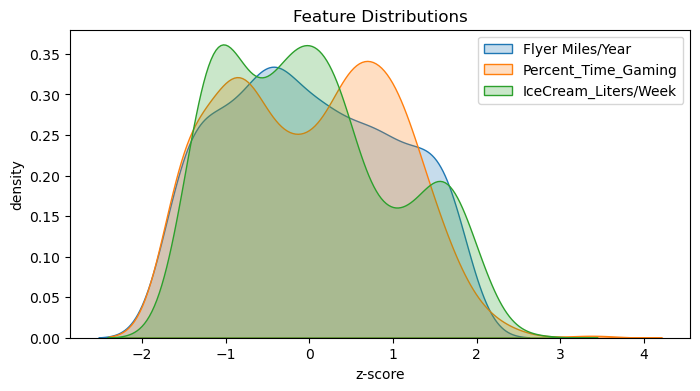
\includegraphics[width=0.65\textwidth, height=0.25\textheight]{pre_a.png}
        \caption{\small{Standardized Distributions}}
    \end{figure}
    \begin{figure}[H]
        \centering
        \begin{minipage}[t]{0.47\textwidth}
            \centering
            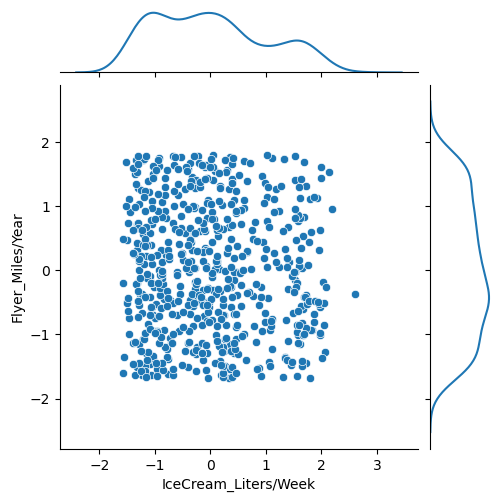
\includegraphics[width=\textwidth, height=0.3\textheight]{pre_c.png}
            \caption{\small{Flyer Miles/Year vs Ice Cream Liters/week}}
        \end{minipage}
        \hfill
        \begin{minipage}[t]{0.47\textwidth}
            \centering
            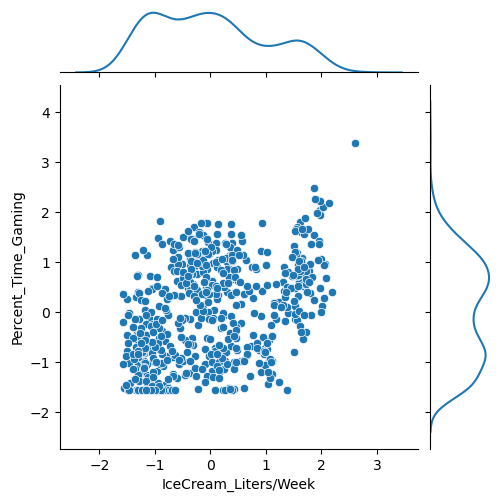
\includegraphics[width=\textwidth, height=0.3\textheight]{pre_b.png}
            \caption{\small{Percentage Time Gaming vs Ice Cream Liters/week}}
        \end{minipage}
    \end{figure}
    \begin{figure}[H]
        \centering
        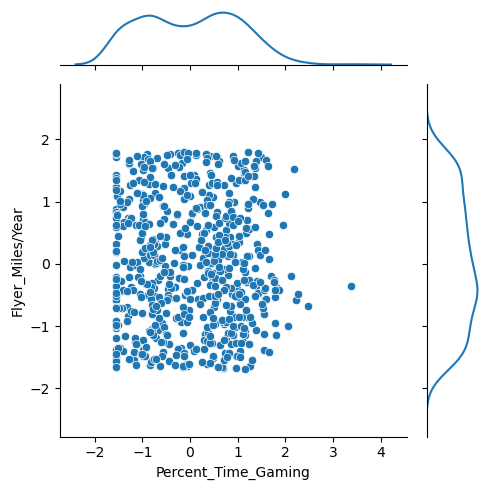
\includegraphics[width=0.47\textwidth, height=0.3\textheight]{pre_d.png}
        \caption{\small{Flyer Miles/Year vs Percentage Time Gaming}}
    \end{figure}

    We can also define a general cross validation helper function and store frequent performance
    metrics in a dictionary:

    \begin{figure}[H]
        \centering
        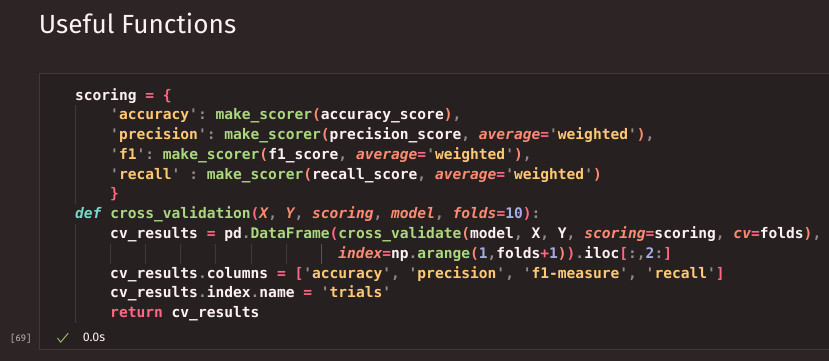
\includegraphics[width=0.65\textwidth, height=0.22\textheight]{helper.png}
        \caption{\small{Utility Functions}}
    \end{figure}

    The following analysis will involve model selection and validation using only
    the \textbf{training dataset}, and then conclude with a final model comparison
    where the selected models are first trained on the \textbf{training set}, and then
    evaluated using the \textbf{test set}.

    \newpage

\section*{Naive Bayes Classification (Gaussian Distribution)}

    \subsection*{Validation}

    Although some correlation can be observed between \textbf{Percentage Time Gaming} and
    \textbf{Ice Cream Liters/week}, Gaussian Naive Bayes remains a robust classification method due to
    roughly normal feature distributions and week/nonexistent overall feature pair correlations indicating
    high degree of feature independence.

    \begin{figure}[H]
        \centering
        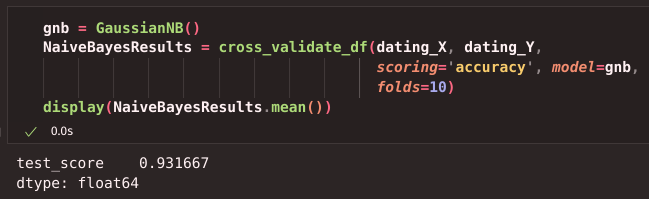
\includegraphics[width=0.7\textwidth, height=0.25\textheight]{NB_results.png}
        \caption{\small{Naive Bayes Cross Validation Results}}
    \end{figure}

\section*{K-NN Classification}

    \subsection*{Model Selection}

    We evaluate the accuracy for k-NN models using different \textbf{k} values. The train/test
    split uses the training data and is shuffled for each of 1000 epochs during which we record model test accuracy
    for models with values of k $\in [1,30]$. At the end of each epoch, we
    increment the count of the k value associated with the highest accuracy score during
    that epoch. The final distribution shows that $k=3$ has the highest accuracy an overwhelming
    majority of the time, and thus we choose $k=3$ as our hyperparameter.
    
    \begin{figure}[H]
        \centering
        \begin{minipage}[t]{0.45\textwidth}
            \centering
            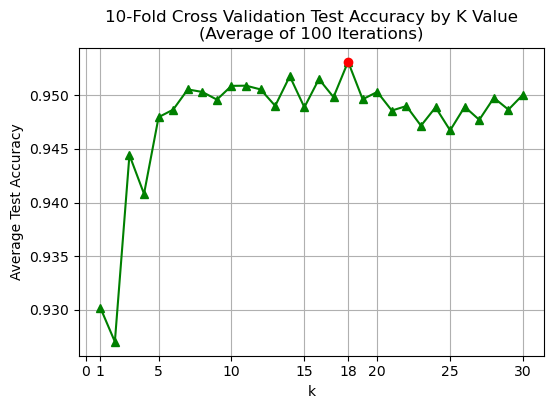
\includegraphics[width=\textwidth, height=0.2\textheight]{k-NN_selection.png}
            \caption{\small{Best K Hyperparameter Selection Barplot}}
        \end{minipage}
        \hfill
        \begin{minipage}[t]{0.54\textwidth}
            \centering
            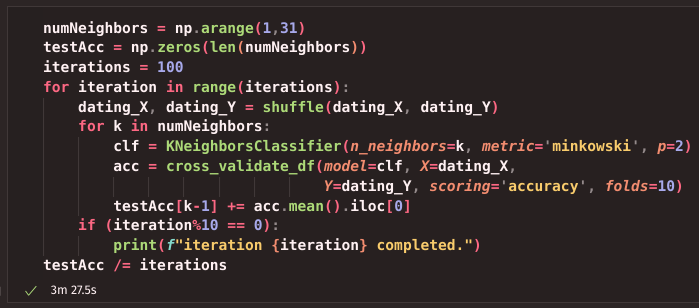
\includegraphics[width=\textwidth, height=0.25\textheight]{k-NN_selection_code.png}
            \caption{\small{Best K Hyperparameter Selection Code}}
        \end{minipage}
    \end{figure}

    \newpage

    \subsection*{Validation}

    Having selecting our model, we perform a 10-fold cross validation and determine the associated average performance
    metrics.

    \begin{figure}[H]
        \centering
        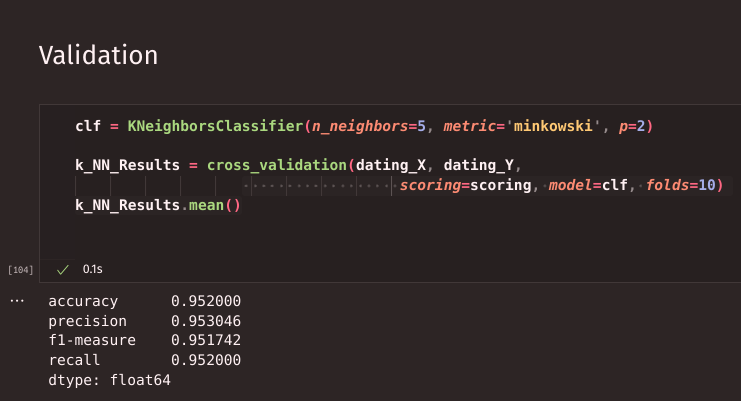
\includegraphics[width=0.7\textwidth, height=0.17\textheight]{k-NN_validation.png}
        \caption{\small{k-NN Cross Validation Results (k=3)}}
    \end{figure}

\section*{Decision Tree Classification}

    \subsection*{Model Selection}

    Using a similar approach as with K-NN classification, we shuffle the data into
    new train/test splits for each of 1000 epochs. During each epoch, we create 
    decision trees of different depths, for both entropy and gini impurity measures.
    For each impurity and depth, we maintain a running total of the test accuracies
    and average these values across the 1000 epochs at the end of the test. 

    \begin{figure}[H]
        \centering
        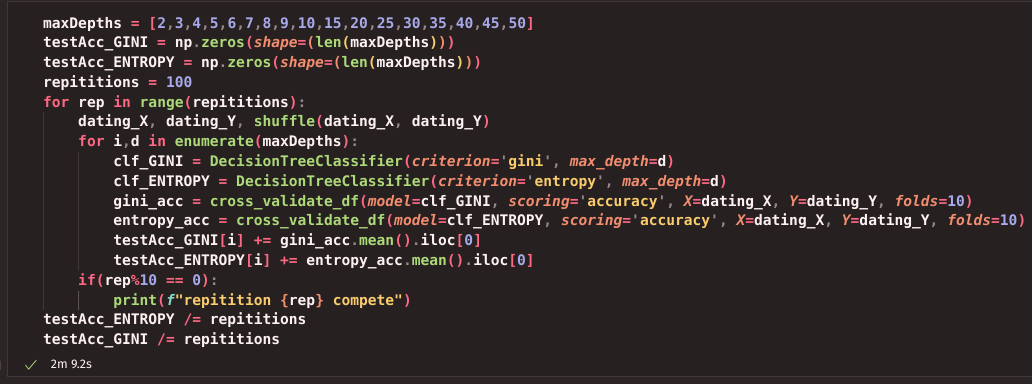
\includegraphics[width=0.7\textwidth, height=0.18\textheight]{tree_selection_code.png}
        \caption{\small{Decision Tree Model Selection Code}}
    \end{figure}
    \begin{figure}[H]
        \centering
        \begin{minipage}[t]{0.49\textwidth}
            \centering
            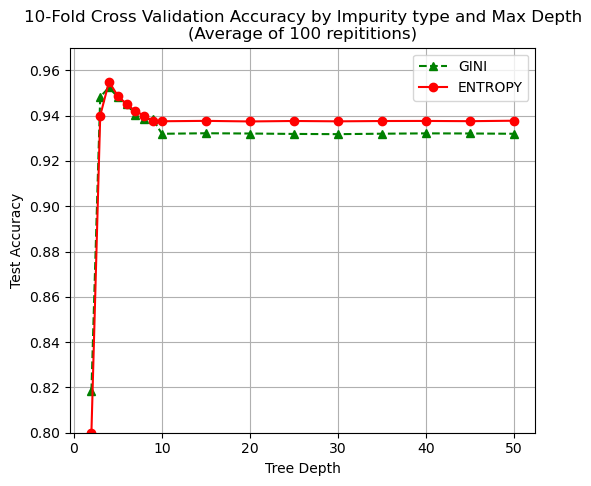
\includegraphics[width=\textwidth, height=0.25\textheight]{tree_selection1.png}
            \caption{\small{Accuracy by Impurity Measure and Depth}}
        \end{minipage}
        \hfill
        \begin{minipage}[t]{0.49\textwidth}
            \centering
            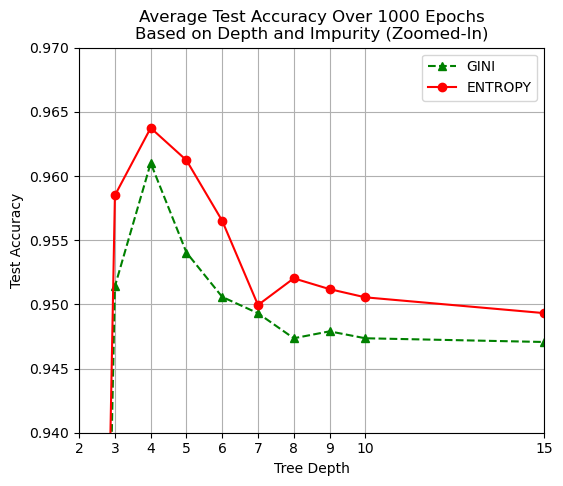
\includegraphics[width=\textwidth, height=0.25\textheight]{tree_selection2.png}
            \caption{\small{Accuracy by Impurity Measure and Depth (Zoomed-In)}}
        \end{minipage}
    \end{figure}

    \newpage

    \subsection*{Validation}

    We see that entropy impurity with a max tree depth of 4 gives the highest test
    accuracy score.

    \begin{figure}[H]
        \centering
        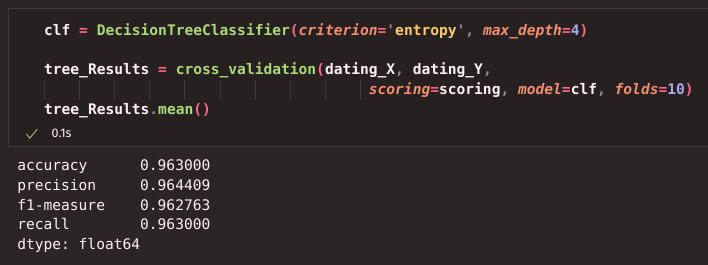
\includegraphics[width=0.7\textwidth, height=0.17\textheight]{tree_validation.png}
        \caption{\small{Decision Tree Validation (Entropy Impurity \& Depth = 4)}}
    \end{figure}

\section*{Test Set Validation}

    \subsection*{Validation}

    Although some correlation can be observed between \textbf{Percentage Time Gaming} and
    \textbf{Ice Cream Liters/week}, Gaussian Naive Bayes remains a robust classification method due to
    roughly normal feature distributions and week/nonexistent overall feature pair correlations indicating
    high degree of feature independence.

    \begin{figure}[H]
        \centering
        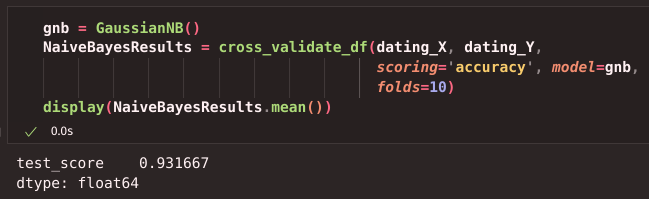
\includegraphics[width=0.7\textwidth, height=0.25\textheight]{NB_results.png}
        \caption{\small{Naive Bayes Cross Validation Results}}
    \end{figure}

\end{document}